% ***********************************************************************************
% Pure LaTeX part to be inserted in a document (be careful of depencies of packages & commands
% Prepared by XXX and YYY under the supervision of Arnaud de La Fortelle
% Fall 2017
% 2D wave propagation subsection of the modeling part
% ***********************************************************************************

\subgroup{4}{Carlin Liao}

\paragraph{Description}
Consider a particle in a discrete two-dimensional grid at location $\vec{x}=[x_1,x_2]$ that moves in discrete time intervals. On each movement, the particle has an equal probability of moving one unit in any of the four cardinal directions $[x_1+1,x_2]$, $[x_1-1,x_2]$, $[x_1,x_2+1]$, and $[x_1,x_2-1]$. Our goal is to describe the probability of the point arriving at point $\vec{x}$ at time $t+1$, $P[\vec{x},t+1]$ using Fick's Law.

% \usepackage{tikz}
\begin{figure}[htb]
\centering
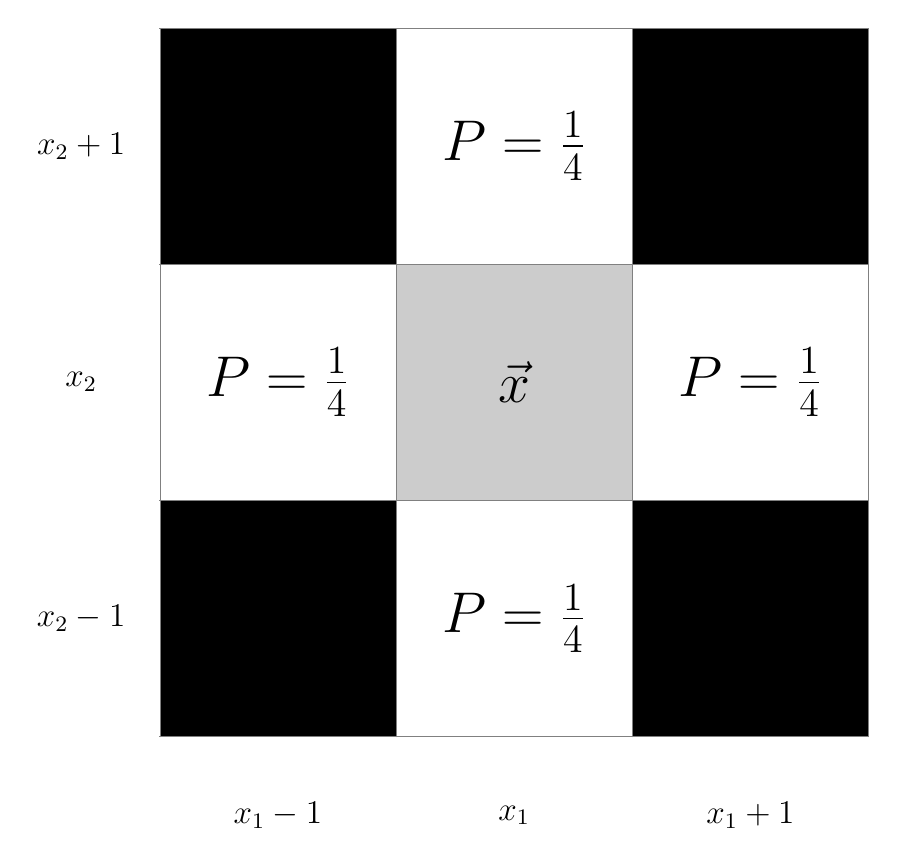
\begin{tikzpicture}

\fill[black] (-3,-3) rectangle (0,0);
\fill[black] (3,3) rectangle (6,6);
\fill[black] (-3,3) rectangle (0,6);
\fill[black] (3,-3) rectangle (6,0);
\fill[gray!40!white] (0,0) rectangle (3,3);

\draw[step=3cm,gray,very thin] (-3.01,-3.01) grid (6,6);

% \node at (1.5,1.5) {\huge$(x_1,x_2)$};
\node at (1.5,1.5) {\huge$\vec{x}$};
\node at (-1.5,1.5) {\huge$P=\frac{1}{4}$};
\node at (1.5,-1.5) {\huge$P=\frac{1}{4}$};
\node at (1.5,4.5) {\huge$P=\frac{1}{4}$};
\node at (4.5,1.5) {\huge$P=\frac{1}{4}$};

\node at (-4,4.5) {\large\bf$x_2+1$};
\node at (-4,1.5) {\large\bf$x_2$};
\node at (-4,-1.5) {\large\bf$x_2-1$};

\node at (-1.5,-4) {\large\bf$x_1-1$};
\node at (1.5,-4) {\large\bf$x_1$};
\node at (4.5,-4) {\large\bf$x_1+1$};

\end{tikzpicture}
\caption{Probability of next step in the 2D random walk}\label{2DrandomWalkProbs.fig}
\end{figure}
    
\paragraph{Model}
Ultimately, our goal is to find a form of Fick's Law using $p(\vec{x},t) = P[\vec{x},t]$, of which the above description is setup for. Note that we can replace $t$ with $t+1$ or any other $t$ without loss of generality due to the memoryless property of 2D random walk.

We begin by describing $P[\vec{x},t+1]$ using our knowledge of the probabilities of where it may be at the prior time step $t$.

\begin{align*}
    P\left[\vec{x}, t+1\right] =&\quad\, \frac{1}{4}P\left[\begin{bmatrix} x_1+1\\x_2 \end{bmatrix}, t\right]\\
    &+\frac{1}{4}P\left[\begin{bmatrix} x_1-1\\x_2 \end{bmatrix}, t\right]\\
    &+\frac{1}{4}P\left[\begin{bmatrix} x_1\\x_2+1 \end{bmatrix}, t\right]\\
    &+\frac{1}{4}P\left[\begin{bmatrix} x_1\\x_2-1 \end{bmatrix}, t\right]
\end{align*}

In order to develop the parallels to Fick's law, we take the Taylor expansions of each of our probabilities with respect to $t$ for $P\left[\vec{x}, t+1\right]$ and with respect to $x$ for each of the probabilities we've used at time $t$.

First, we take the our target probability and find its first order Taylor expansion with respect to time, and using our $p(\vec{x},t)$ as described earlier.
\begin{align*}
    P\left[\vec{x}, t+1\right] &\approx P\left[\vec{x}, t+1\right] + \nabla^T_t\left(P\left[\vec{x}, t+1\right]\right) (t+1-t) \\
    &= p + \frac{\partial p}{\partial t} \\
    &= p
\end{align*}
Note that we exploit the memoryless property of random walk to reduce $\frac{\partial p}{\partial t}$ to 0, as the probability that a particle performing truly random walk is in a certain location in space is not influenced by time.

Next, we take the second order Taylor expansion of our probabilities of movement in the $x_1$ direction, using similar substitutions as before. Here, $\mathcal{H}(f)$ describes the Hessian of the function $f$. 
\begin{align*}
    P\left[\begin{bmatrix} x_1\pm1\\x_2 \end{bmatrix}, t\right] &\approx p + \nabla^T_{\vec{x}}(p) \left(\begin{bmatrix} x_1\pm1\\x_2 \end{bmatrix} - \vec{x}\right) + \left(\begin{bmatrix} x_1\pm1\\x_2 \end{bmatrix} - \vec{x}\right)^T \mathcal{H}(p)  \left(\begin{bmatrix} x_1\pm1\\x_2 \end{bmatrix} - \vec{x}\right) \\
    &= p + \left(\frac{\partial p}{\partial x}\right)^T \begin{bmatrix} \pm1\\0 \end{bmatrix} + \begin{bmatrix} \pm1\\0 \end{bmatrix}^T \begin{bmatrix}
        \frac{\partial^2 p}{\partial x_1^2} & \frac{\partial p}{\partial x_2 x_1} \\
        \frac{\partial p}{\partial x_1 x_2} & \frac{\partial^2 p}{\partial x_2^2}
    \end{bmatrix} \begin{bmatrix} \pm1\\0 \end{bmatrix} \\
    &= p \pm \left(\frac{\partial p}{\partial x}\right)^T \begin{bmatrix} 1\\0 \end{bmatrix} + \frac{\partial^2 p}{\partial x_1^2}
\end{align*}

Similarly, we take the second order Taylor expansion for probabilities in the $x_2$ direction.
\begin{align*}
    P\left[\begin{bmatrix} x_1\\x_2\pm1 \end{bmatrix}, t\right] &\approx 
    p + 
    \nabla^T_{\vec{x}}(p) \left(\begin{bmatrix} x_1\\x_2\pm1 \end{bmatrix} - \vec{x}\right) + \left(\begin{bmatrix} x_1\\x_2\pm1 \end{bmatrix} - \vec{x}\right)^T \mathcal{H}(p)  \left(\begin{bmatrix} x_1\\x_2\pm1 \end{bmatrix} - \vec{x}\right) \\
    &= p \pm \left(\frac{\partial p}{\partial x}\right)^T \begin{bmatrix} 0\\1 \end{bmatrix} + \begin{bmatrix} 0\\1 \end{bmatrix}^T \begin{bmatrix}
        \frac{\partial^2 p}{\partial x_1^2} & \frac{\partial p}{\partial x_2 x_1} \\
        \frac{\partial p}{\partial x_1 x_2} & \frac{\partial^2 p}{\partial x_2^2}
    \end{bmatrix} \begin{bmatrix} 0\\1 \end{bmatrix} \\
    &= p \pm \left(\frac{\partial p}{\partial x}\right)^T \begin{bmatrix} 0\\1 \end{bmatrix} + \frac{\partial^2 p}{\partial x_2^2}
\end{align*}

Now, we combine all of the above into our original expression
\begin{align*}
    p =&\quad\, \frac{1}{4}\left(p + \left(\frac{\partial p}{\partial x}\right)^T \begin{bmatrix} 1\\0 \end{bmatrix} + \frac{\partial^2 p}{\partial x_1^2}\right)\\
    &+\frac{1}{4}\left(p - \left(\frac{\partial p}{\partial x}\right)^T \begin{bmatrix} 1\\0 \end{bmatrix} + \frac{\partial^2 p}{\partial x_1^2}\right)\\
    &+\frac{1}{4}\left(p + \left(\frac{\partial p}{\partial x}\right)^T \begin{bmatrix} 0\\1 \end{bmatrix} + \frac{\partial^2 p}{\partial x_2^2}\right)\\
    &+\frac{1}{4}\left(p - \left(\frac{\partial p}{\partial x}\right)^T \begin{bmatrix} 0\\1 \end{bmatrix} + \frac{\partial^2 p}{\partial x_2^2}\right)
\end{align*}
We note how the first order terms cancel out and proceed to further simplify. Take note of the use of the Laplacian operator $\nabla^2$.
\begin{align*}
    p &= p + \frac{1}{4}\left(\frac{\partial^2 p}{\partial x_1^2}+\frac{\partial^2 p}{\partial x_1^2}+\frac{\partial^2 p}{\partial x_2^2}+\frac{\partial^2 p}{\partial x_2^2}\right) \\
    0 &= \frac{1}{2}\left(\frac{\partial^2 p}{\partial x_1^2}+\frac{\partial^2 p}{\partial x_2^2}\right)\\
    \nabla^2 p &= \frac{\partial^2 p}{\partial x_1^2}+\frac{\partial^2 p}{\partial x_2^2}\\
    \nabla^2 p &= 0
\end{align*}
We note that this final result to be (as expected) the solution to Fick's second law in the special case of the diffusion (or random walk, in our case) being independent of time, also known as Laplace's equation. For a more general result (i.e. not assuming that our particle's position is independent of time), using these same methods we would arrive at the more general statement of Fick's second law
$$\frac{\partial p}{\partial t} = \nabla^2 p$$

To close, while this result was derived for the two-dimensional random walk case, the derivation for n-dimensions should be readily apparent from this case.


\vspace{12pt}


{\it Adapted in part from} \url{http://engineering.dartmouth.edu/~d30345d/courses/engs43/chapter2.pdf}